\section{Background modeling}
\label{sec:BkgModeling}

\subsection{Blind strategy}
\label{subsec:BlindStrategy}
In the following sections, modeling of kinematic distributions, in particular ones used for BDT training, of the $t\bar{t}+\text{jets}$ background is checked by comparing the data and MC. In order to avoid observing signals or any other biases before fixing the analysis procedure, following blinding strategy is applied. The signal to noise ratio ($S/B$) is calculated in each bin of each distribuion on for all $H^{+}$ mass hypothesis (more details in Appendix \ref{app:SignalBackgroundComparison}). The signal cross section (${\sigma}_{\text{signal}}$) on each $H^{+}$ mass hypothesis is set to 0.046 pb, which is the upper limits at 1 TeV $H^{+}$ mass point obtained from the resolved $H^{+}{\rightarrow}tb$ search \cite{HDBS-2021-02}, and therefore it can be considered as the most conservative assumption. The data in bins with $S/B>0.05$ in at least one $H^{+}$ mass hypothesis are blinded when the data is compared with MC.

%Furthermore, the final BDT distributions input into the profile likehood fits are compared between the data and MC in Section \ref{subsec:Data/MCFinalDiscBeforeReweight}. Before the comparison, S/B is calculated in each bin with on ${\sigma}_{\text{signal}}=0.046$ pb as shown in Appendix \ref{subapp:SOVERB_FinalDiscriminant}. And bins with S/B>0.05 are blinded when the data is compared with MC same as above.

\subsection{Data/MC comparison for BDT input variables}
\label{subsec:Data/MCBDTInputBeforeReweight}
Figures \ref{fig:DATAOVERMC_BDTInputs_Prefit} show the distributions of input variables for BDT training. Data are blinded according to the blind strategy in Section \ref{subsec:BlindStrategy}. No significant difference between the data and MC is found in each variable.

\begin{figure}[H]
  \subfloat[HT\_jets] {
    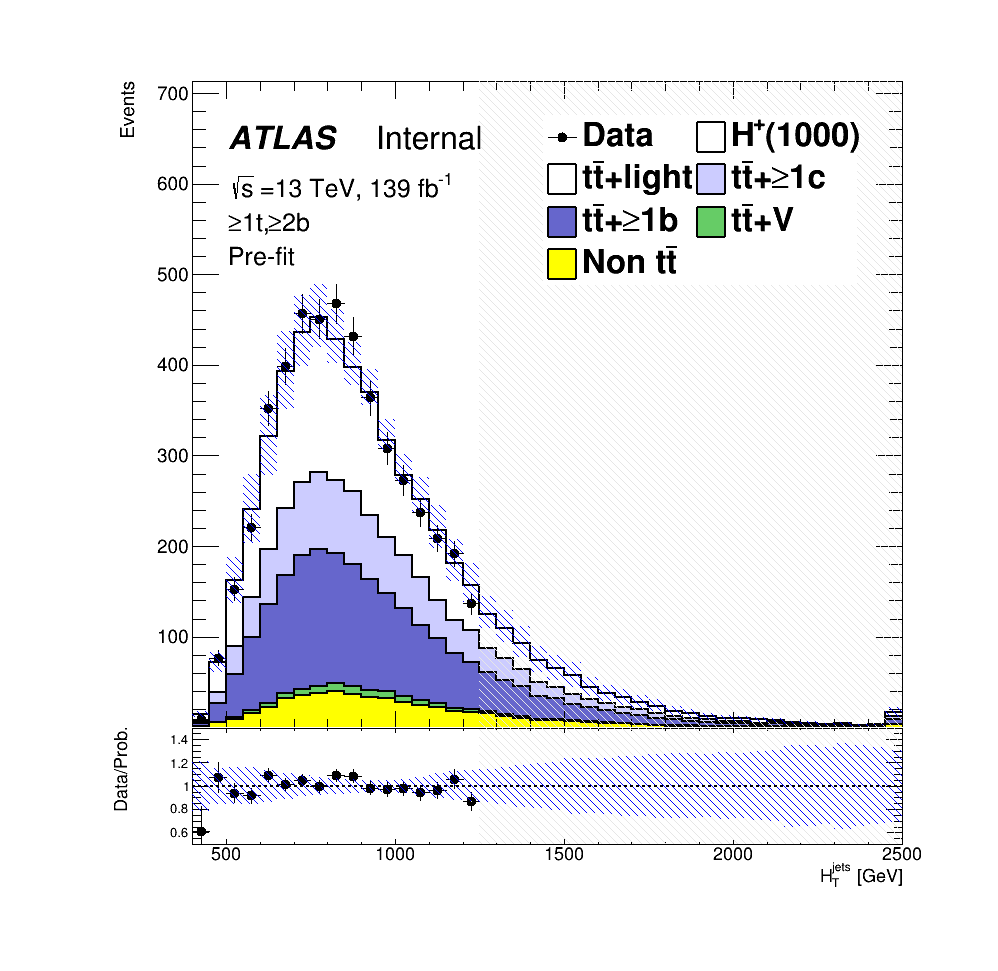
\includegraphics[width=0.25\textwidth]{images/BkgModeling/DATAOVERMC_Hp1000_Contained80_DL1r_70_HT_jets_geq1tgeq2b_prefit.png}
    \label{fig:DATAOVERMC_HT_jets}
  }
  \subfloat[LeadingJet\_pt] {
    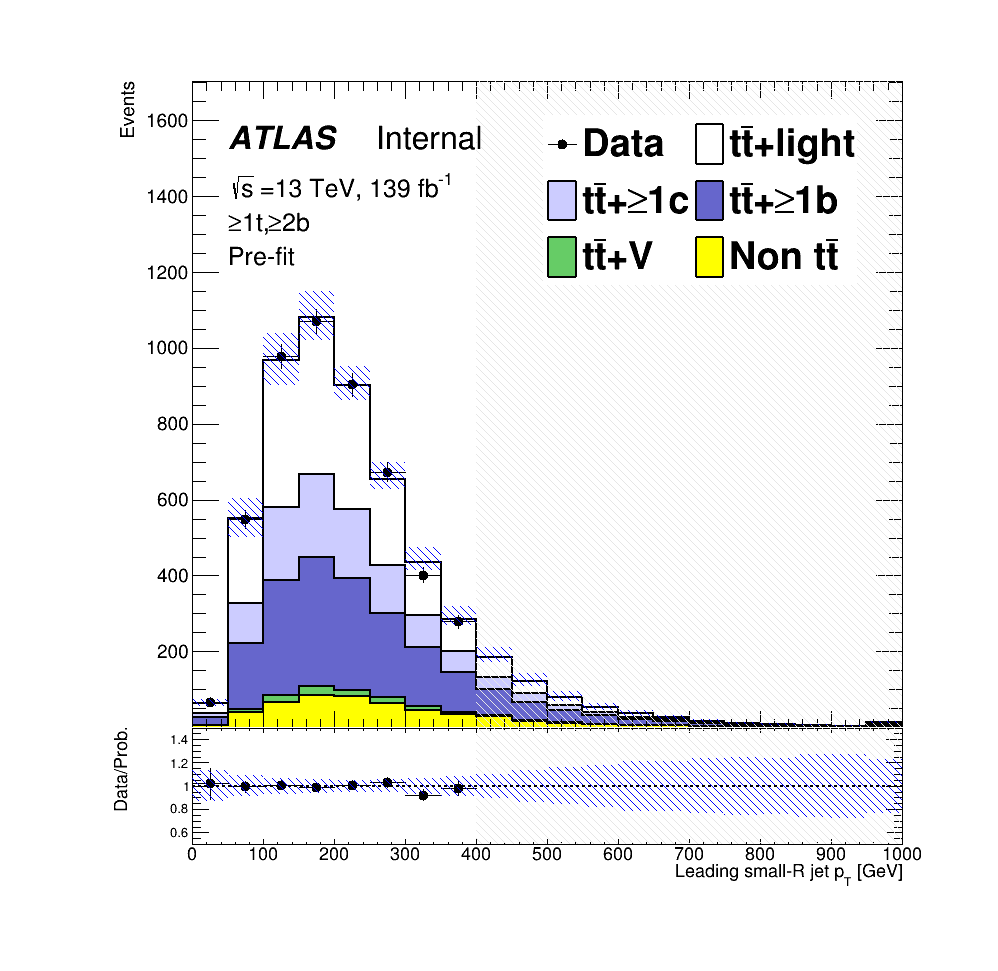
\includegraphics[width=0.25\textwidth]{images/BkgModeling/DATAOVERMC_Hp1000_Contained80_DL1r_70_LeadingJet_pt_geq1tgeq2b_prefit.png}
    \label{fig:DATAOVERMC_LeadingJet_pt}
  }
  \subfloat[Centrality\_all] {
    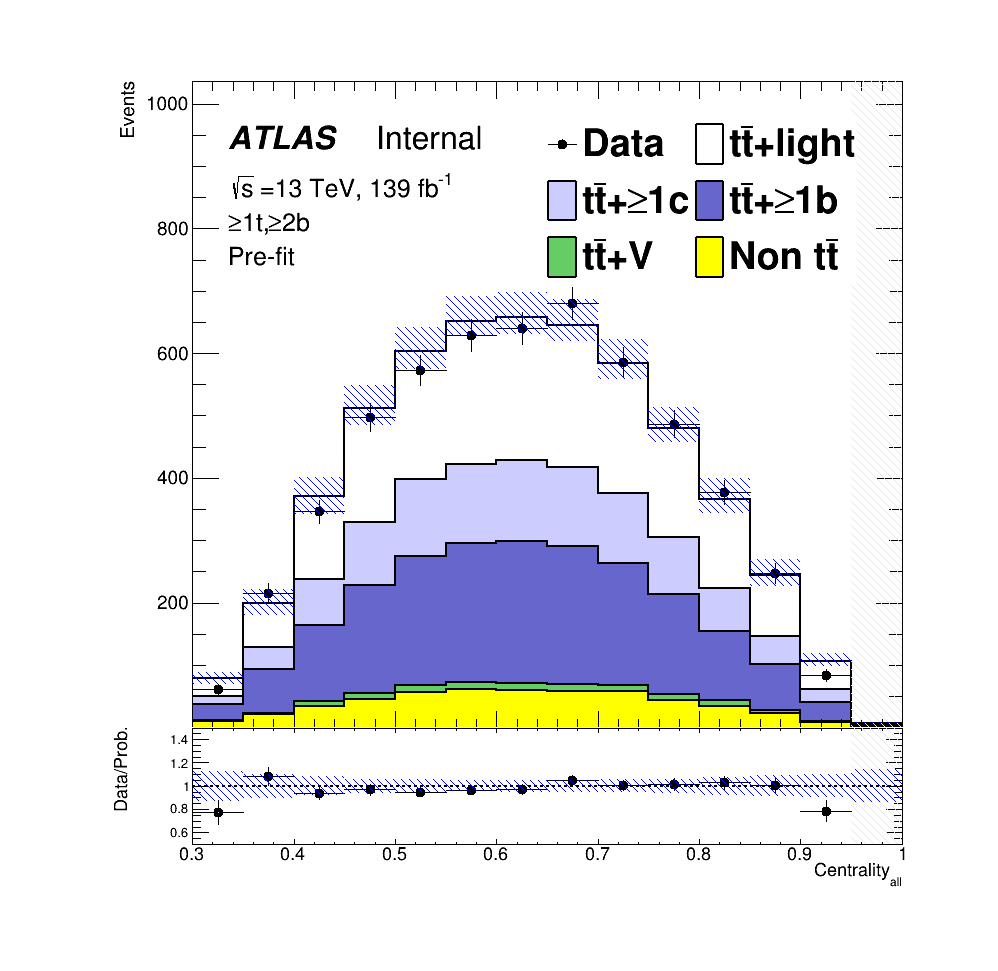
\includegraphics[width=0.25\textwidth]{images/BkgModeling/DATAOVERMC_Hp1000_Contained80_DL1r_70_Centrality_all_geq1tgeq2b_prefit.png}
    \label{fig:DATAOVERMC_Centrality_all}
  }
  \subfloat[H1\_all] {
    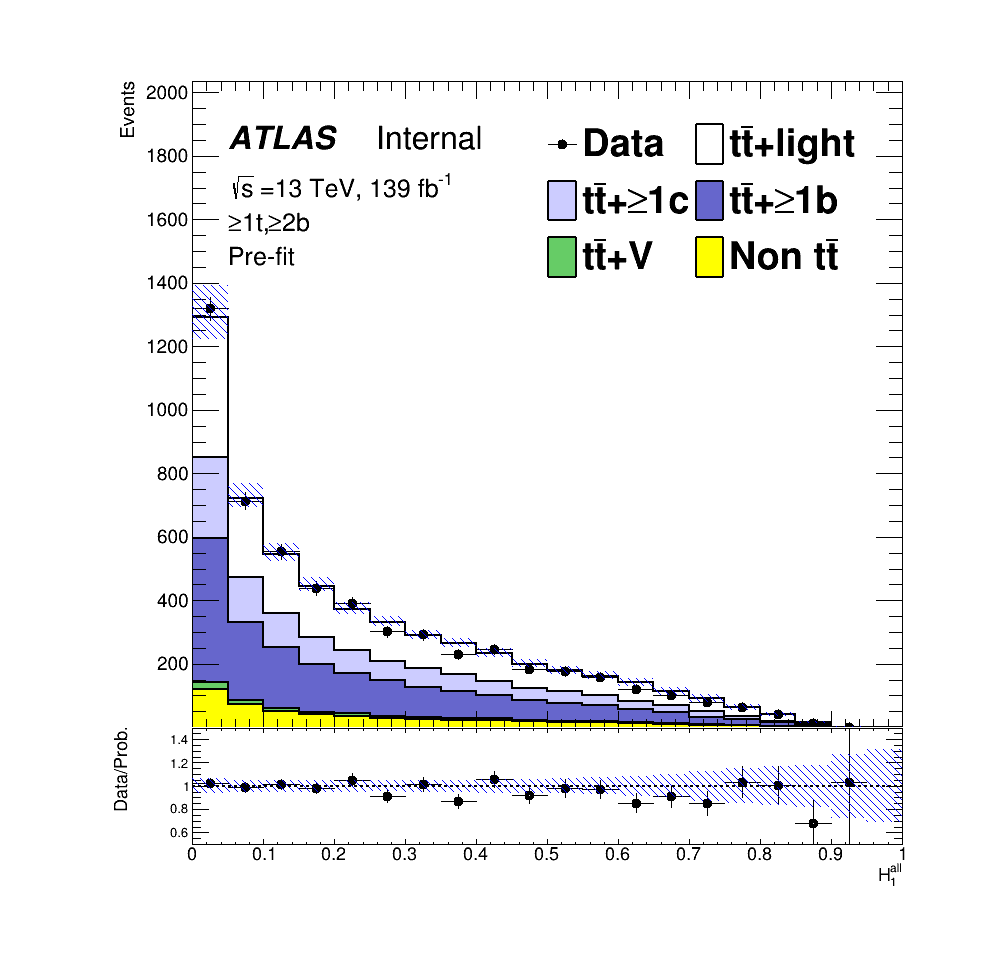
\includegraphics[width=0.25\textwidth]{images/BkgModeling/DATAOVERMC_Hp1000_Contained80_DL1r_70_H1_all_geq1tgeq2b_prefit.png}
    \label{fig:DATAOVERMC_H1_all}
  }\\
  \subfloat[Mbb\_MaxPt] {
    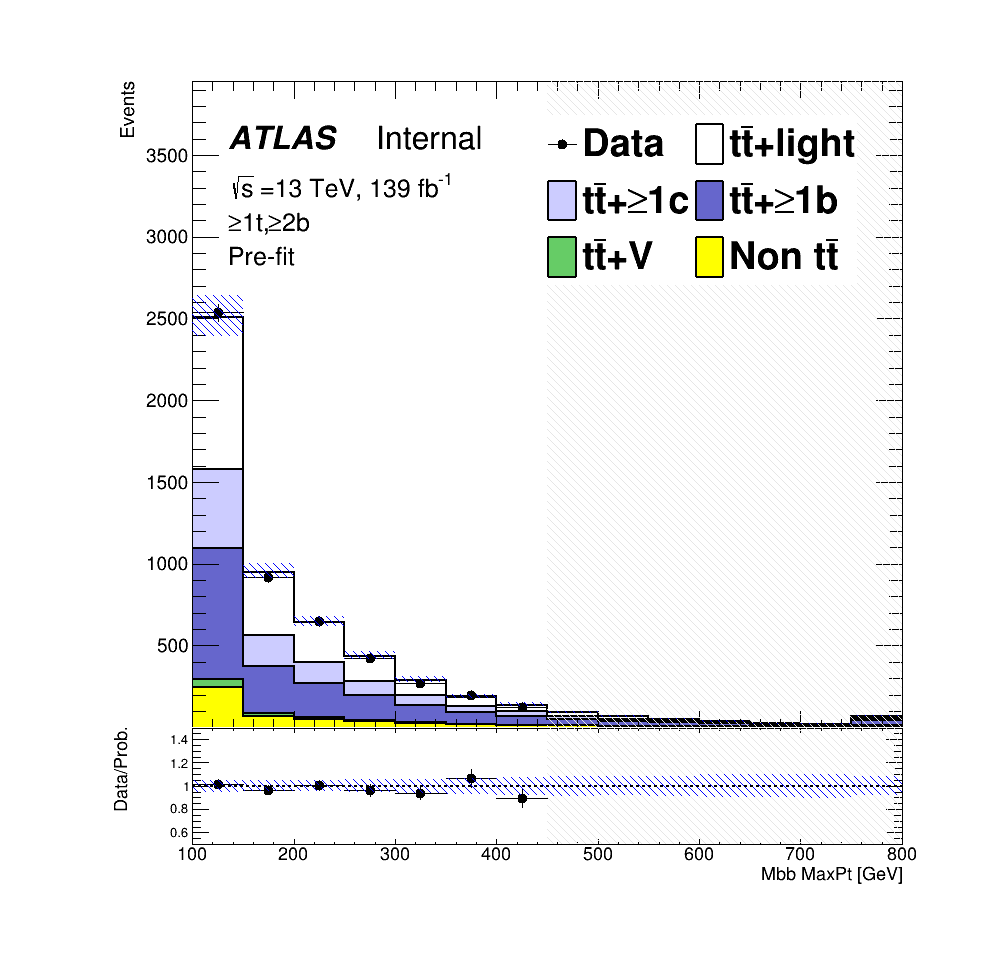
\includegraphics[width=0.25\textwidth]{images/BkgModeling/DATAOVERMC_Hp1000_Contained80_DL1r_70_Mbb_MaxPt_geq1tgeq2b_prefit.png}
    \label{fig:DATAOVERMC_Mbb_MaxPt}
  }
  \subfloat[Mjjj\_MaxPt] {
    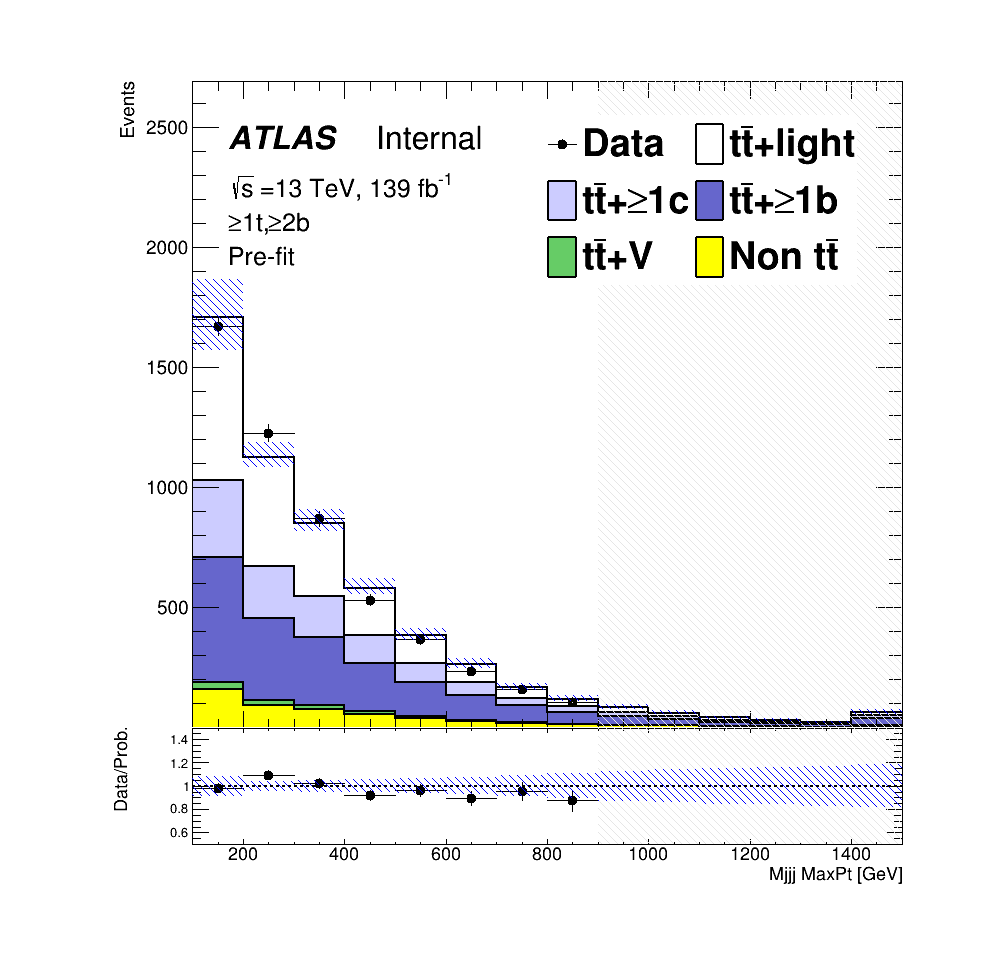
\includegraphics[width=0.25\textwidth]{images/BkgModeling/DATAOVERMC_Hp1000_Contained80_DL1r_70_Mjjj_MaxPt_geq1tgeq2b_prefit.png}
    \label{fig:DATAOVERMC_Mjjj_MaxPt}
  }
  \subfloat[Muu\_MindR] {
    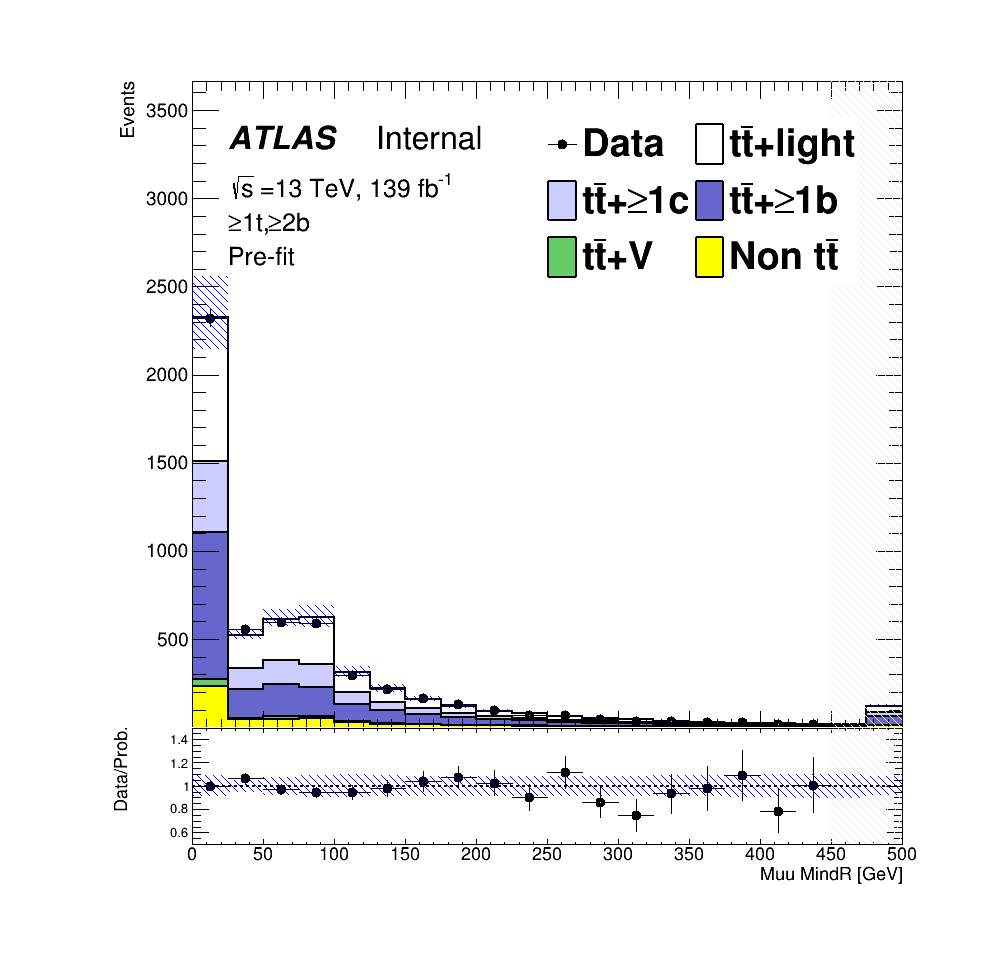
\includegraphics[width=0.25\textwidth]{images/BkgModeling/DATAOVERMC_Hp1000_Contained80_DL1r_70_Muu_MindR_geq1tgeq2b_prefit.png}
    \label{fig:DATAOVERMC_Muu_MindR}
  }
  \subfloat[dRbb\_avg] {
    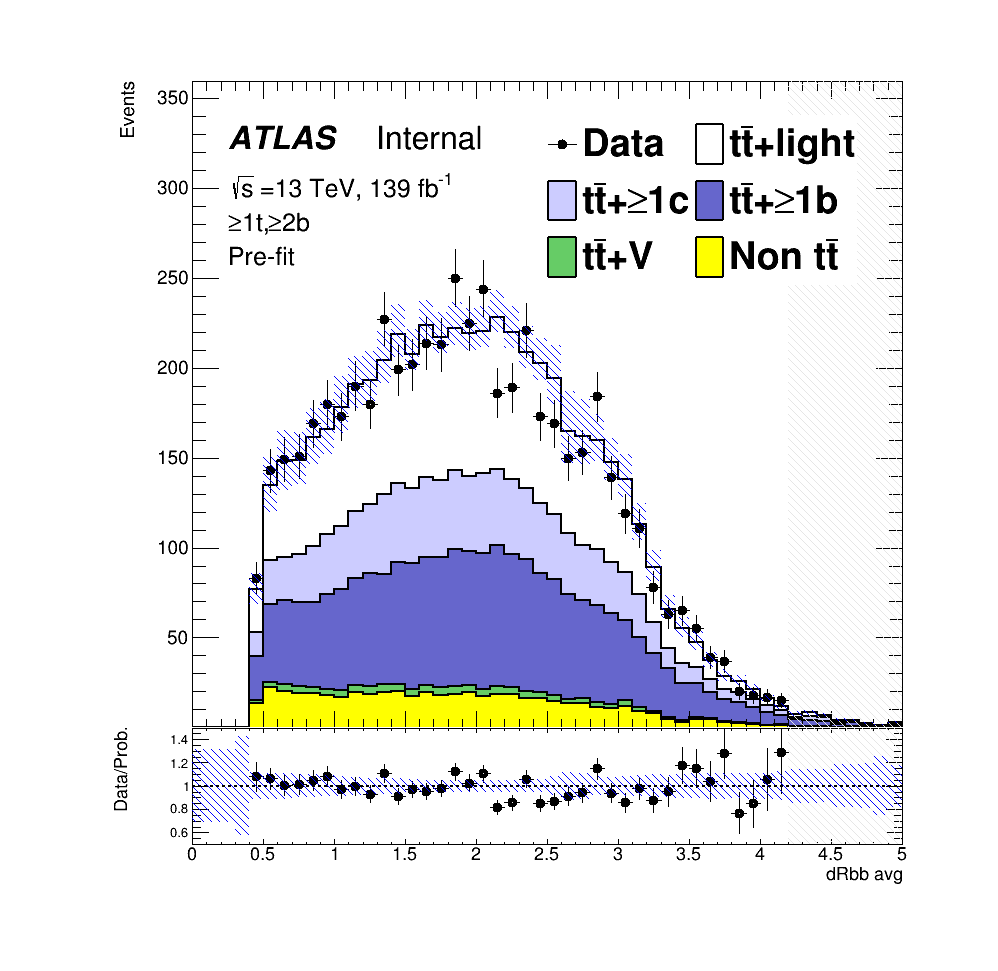
\includegraphics[width=0.25\textwidth]{images/BkgModeling/DATAOVERMC_Hp1000_Contained80_DL1r_70_dRbb_avg_geq1tgeq2b_prefit.png}
    \label{fig:DATAOVERMC_dRbb_avg}
  }\\
  \subfloat[dRlepbb\_MindR] {
    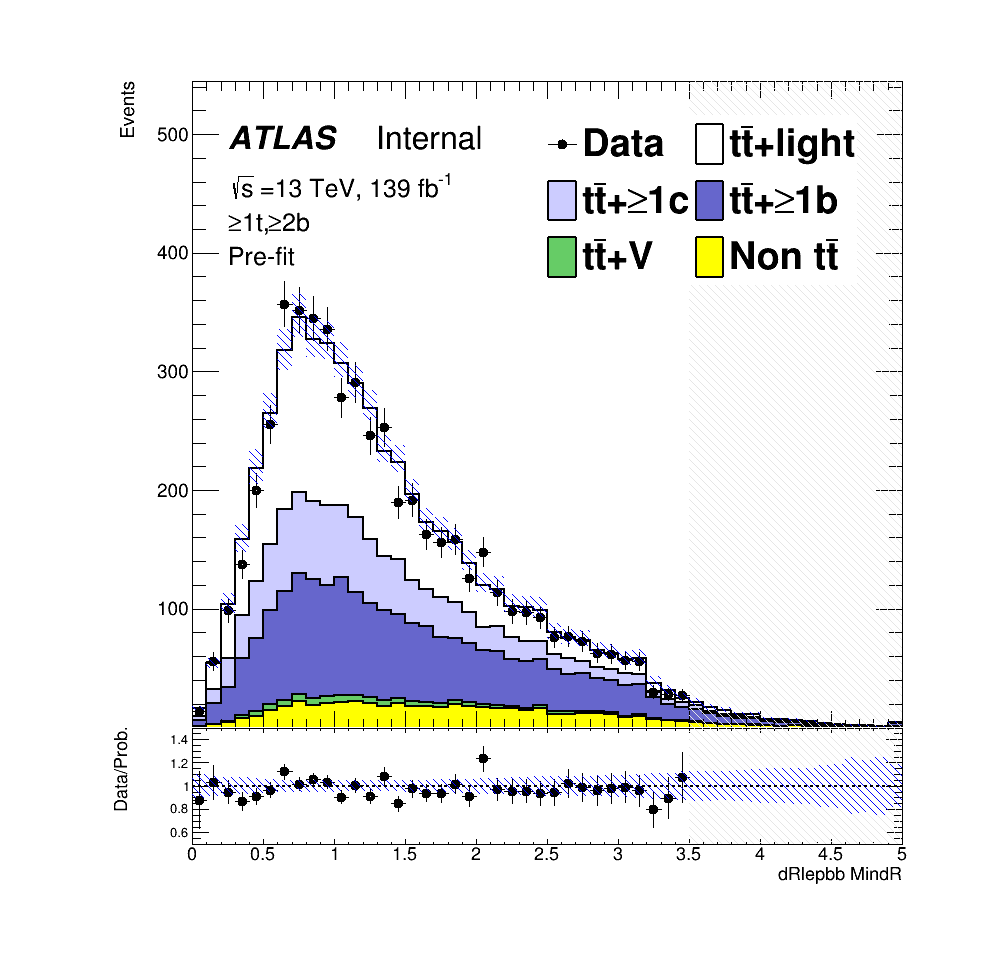
\includegraphics[width=0.25\textwidth]{images/BkgModeling/DATAOVERMC_Hp1000_Contained80_DL1r_70_dRlepbb_MindR_geq1tgeq2b_prefit.png}
    \label{fig:DATAOVERMC_dRlepbb_MindR}
  }
  \subfloat[LeadingTop\_m] {
    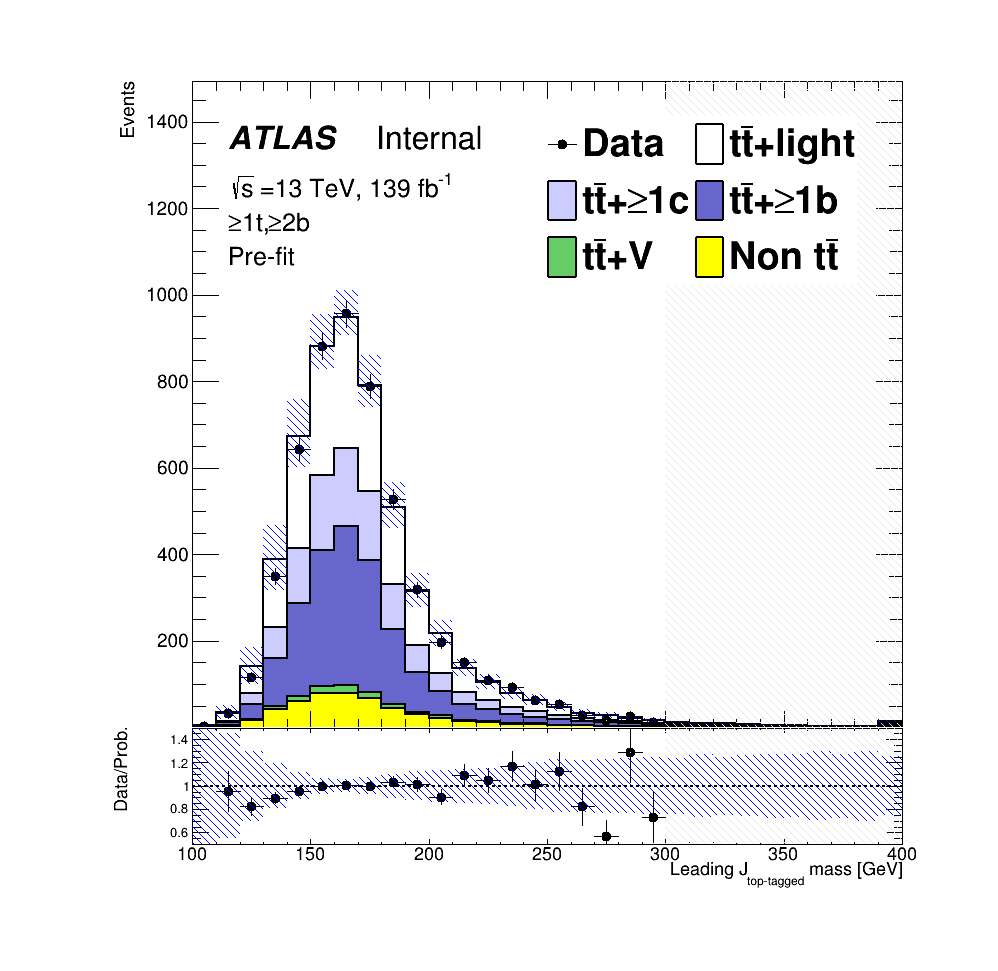
\includegraphics[width=0.25\textwidth]{images/BkgModeling/DATAOVERMC_Hp1000_Contained80_DL1r_70_LeadingTop_mass_geq1tgeq2b_prefit.png}
    \label{fig:DATAOVERMC_LeadingTop_mass}
  }
  \subfloat[LeadingTop\_pt] {
    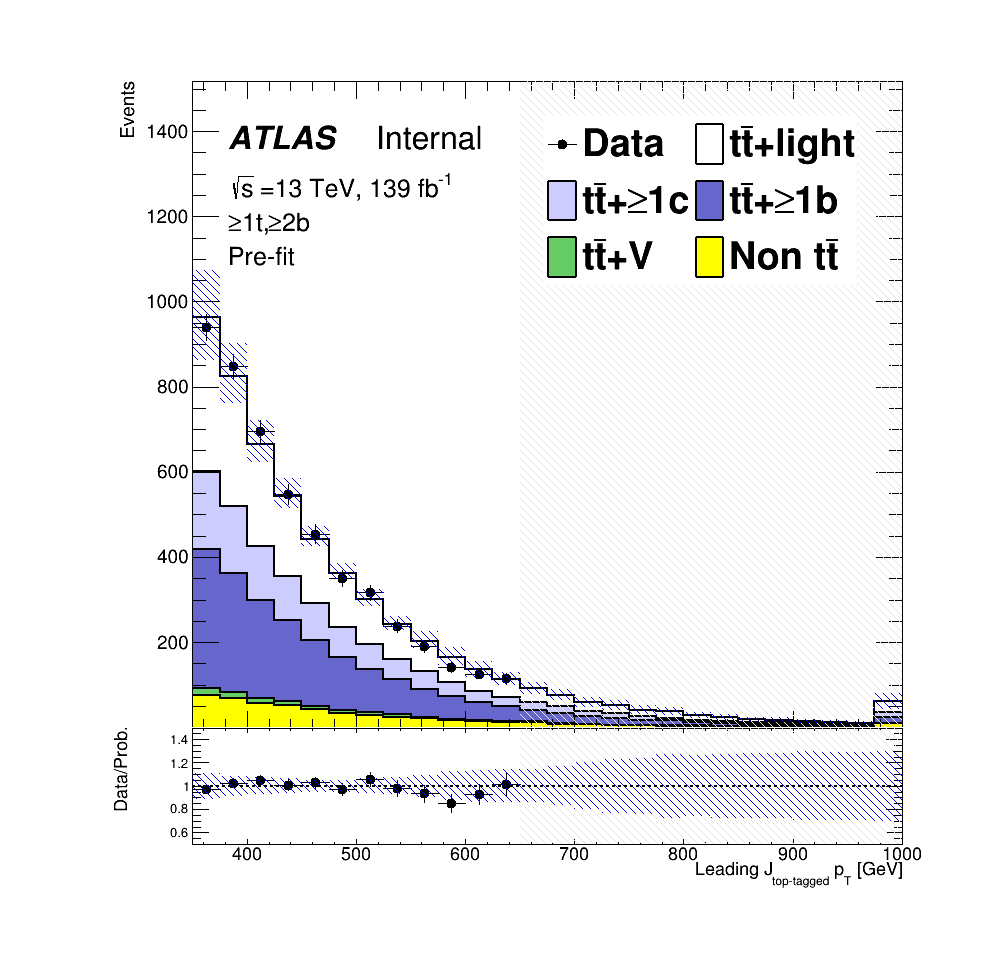
\includegraphics[width=0.25\textwidth]{images/BkgModeling/DATAOVERMC_Hp1000_Contained80_DL1r_70_LeadingTop_pt_geq1tgeq2b_prefit.png}
    \label{fig:DATAOVERMC_LeadingTop_pt}
  }
  \subfloat[M\_tb] {
    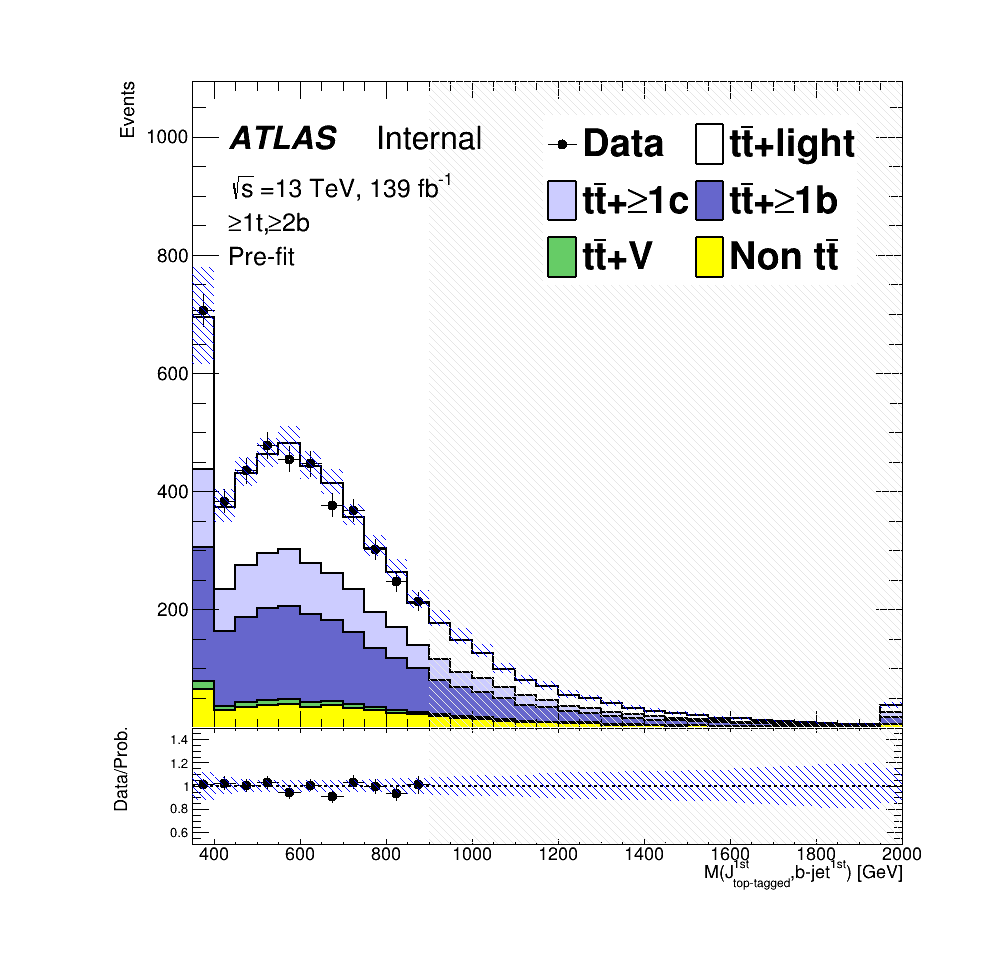
\includegraphics[width=0.25\textwidth]{images/BkgModeling/DATAOVERMC_Hp1000_Contained80_DL1r_70_tb_mass_geq1tgeq2b_prefit.png}
    \label{fig:DATAOVERMC_tb_mass}
  }\\
  \subfloat[Pt\_tb] {
    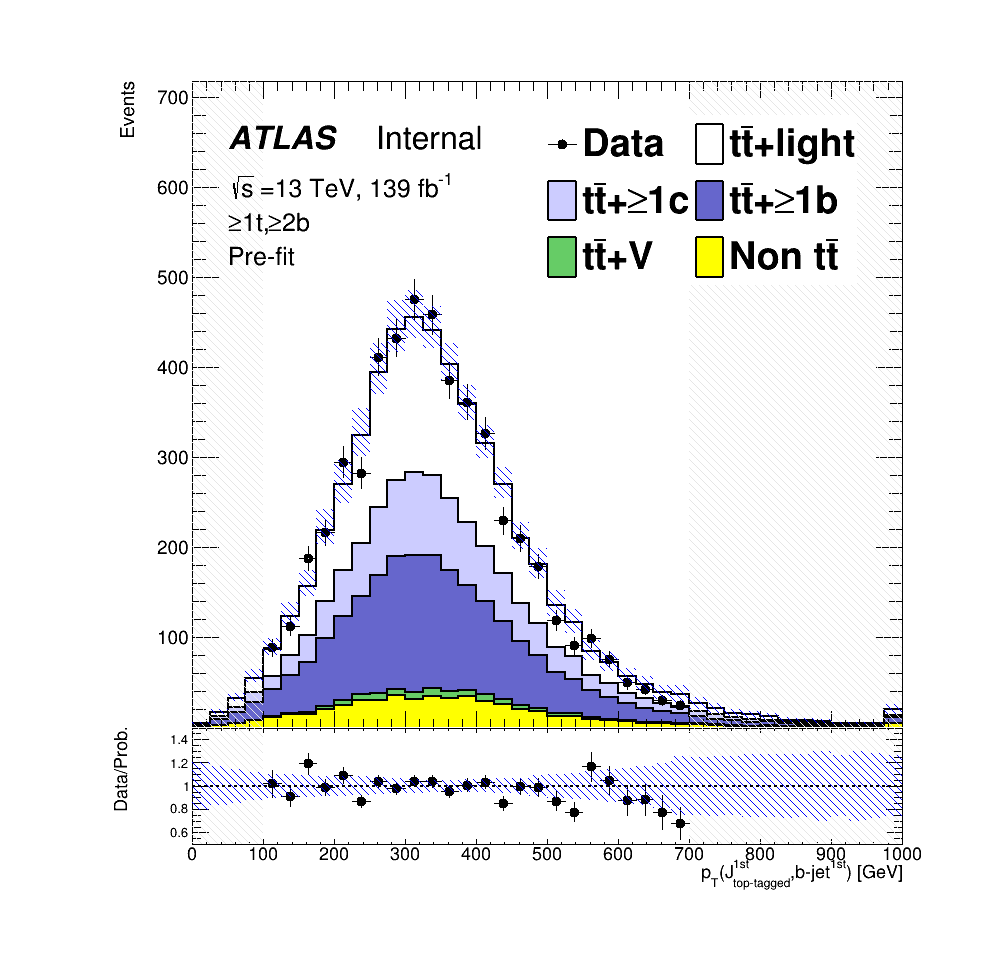
\includegraphics[width=0.25\textwidth]{images/BkgModeling/DATAOVERMC_Hp1000_Contained80_DL1r_70_tb_pt_geq1tgeq2b_prefit.png}
    \label{fig:DATAOVERMC_tb_pt}
  }
  \subfloat[PtAsymm\_tb] {
    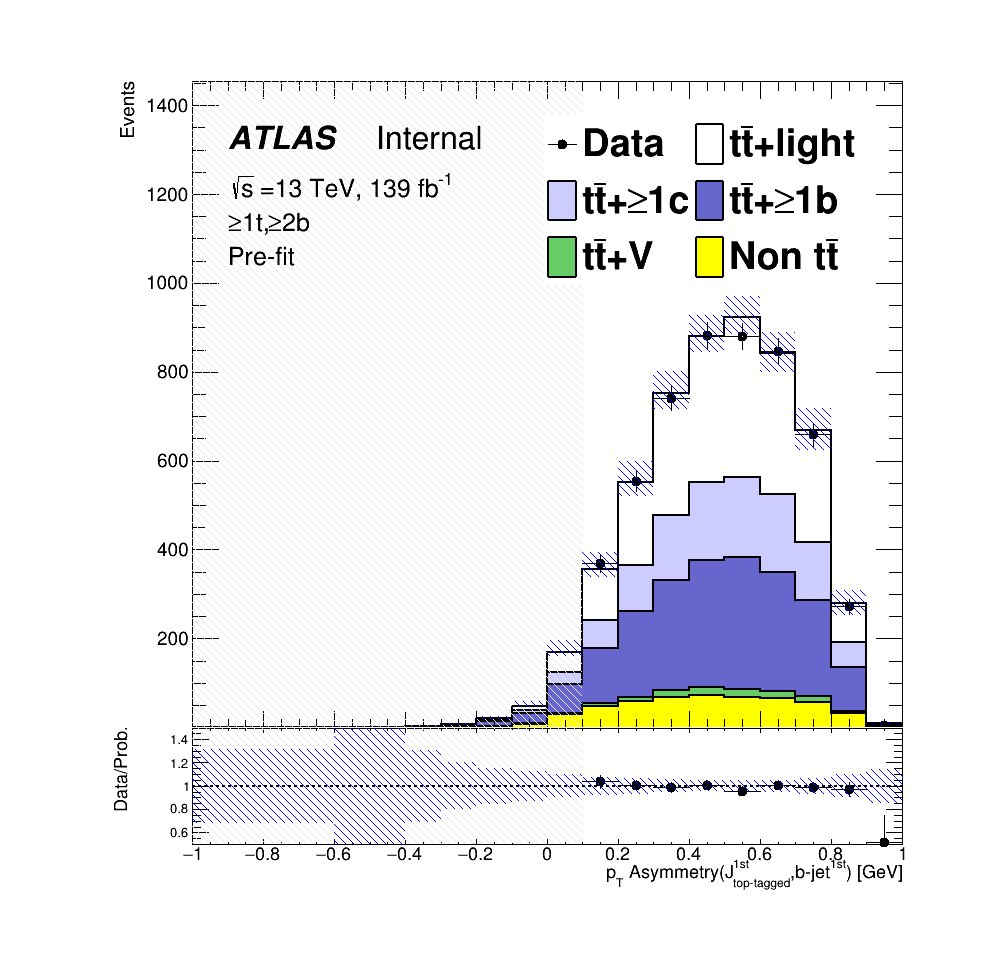
\includegraphics[width=0.25\textwidth]{images/BkgModeling/DATAOVERMC_Hp1000_Contained80_DL1r_70_tb_ptAsymm_geq1tgeq2b_prefit.png}
    \label{fig:DATAOVERMC_tb_ptAsymm}
  }
  \caption{Comparison of the kinematic variables included in the BDT in the SR for the data and MC.}
  \label{fig:DATAOVERMC_BDTInputs_Prefit}
\end{figure}


\subsection{Data/MC comparison for BDT distributions}
\label{subsec:Data/MCFinalDiscBeforeReweight}
Figures \ref{fig:Prefit_Hp1000} to \ref{fig:Prefit_Hp3000} show the distributions of BDT output in SR and $H_{\text{T}}^{\text{jets}}$ in CR. The distributions are input into the profile likelihood fit on each $H^{+}$ mass hypothesis as shown in Section \ref{sec:ProfileLikelohoodFit}. It is observed that the data/MC ratio tends to be lower for the high BDT score regions, which may bias search for the signal in the highest BDT bins. The reweighting to correct for the slope is discussed in Section \ref{subsec:Reweighting}. In $H_{\text{T}}^{\text{jets}}$ distritbutions, there is no significant difference in the shape, while the normalization is significantly different. The $t\bar{t}+\text{light}$ yields are therefore determined by floating them in the fit.

\begin{figure}[H]
  \subfloat[] {
    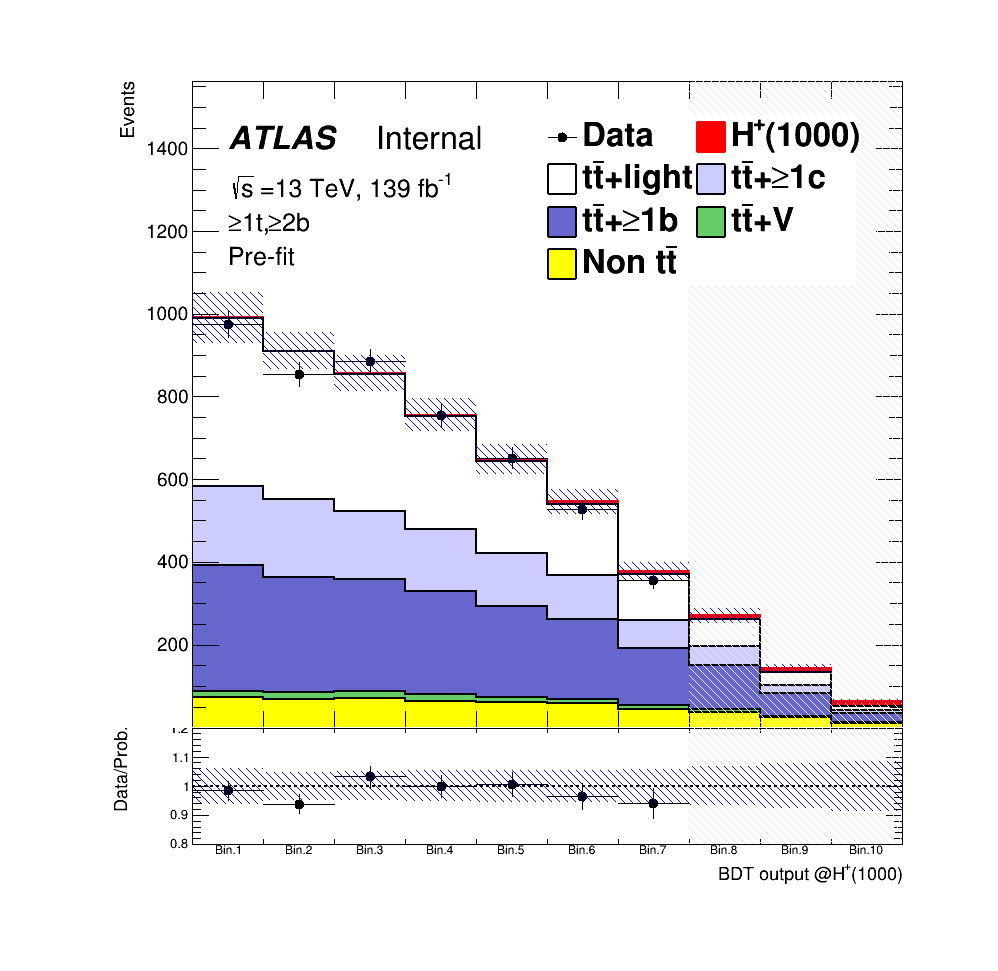
\includegraphics[width=0.50\textwidth]{images/BkgModeling/DATAOVERMC_Hp1000_Contained80_DL1r_70_bdt_Hp1000_geq1tgeq2b_prefit.png}
    \label{fig:Prefit_BDT_Hp1000}
  }
  \subfloat[] {
    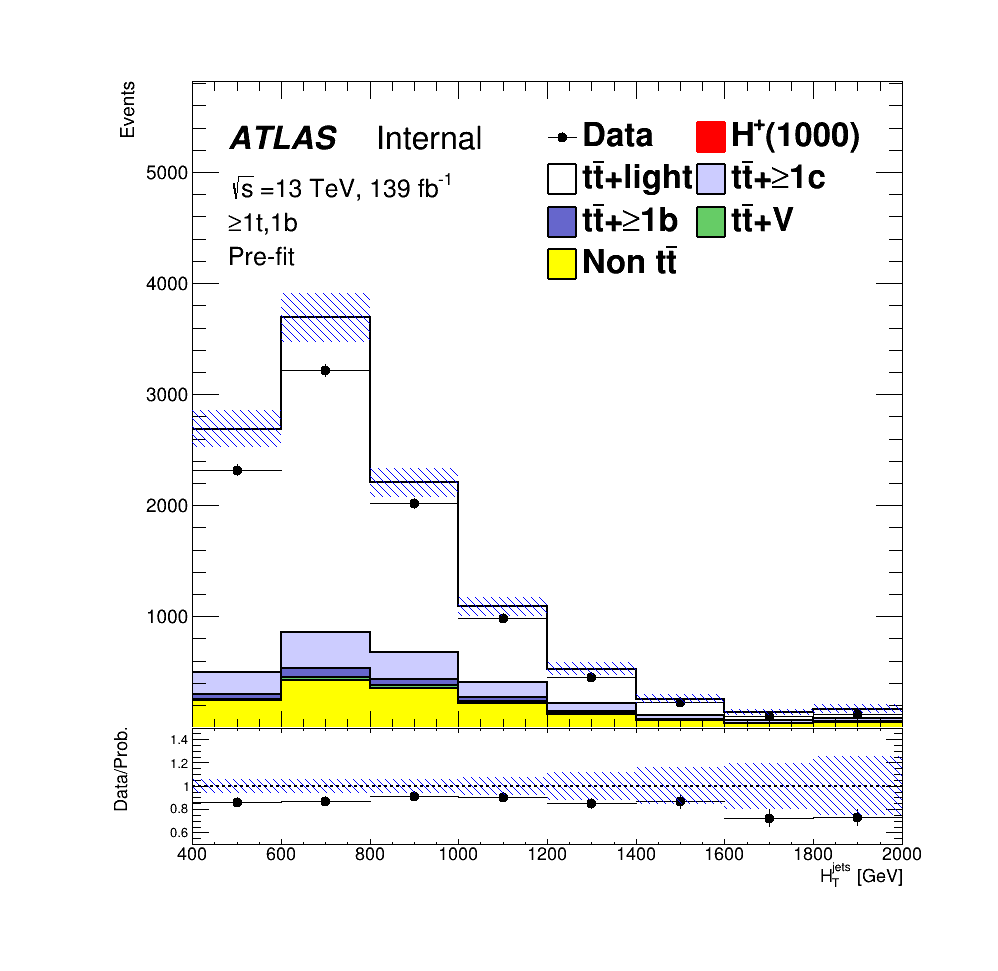
\includegraphics[width=0.50\textwidth]{images/BkgModeling/DATAOVERMC_Hp1000_Contained80_DL1r_70_HT_jets_geq1t1b_prefit.png}
    \label{fig:Prefit_HT_jets_Hp1000}
  }
  \caption{Pre-fit distribution of BDT output in the SR (a) and $H_{\text{T}}^{\text{jets}}$ in the CR for the 1000 GeV $H^{+}$ mass hypotheses.}
  \label{fig:Prefit_Hp1000}
\end{figure}

\begin{figure}[H]
  \subfloat[] {
    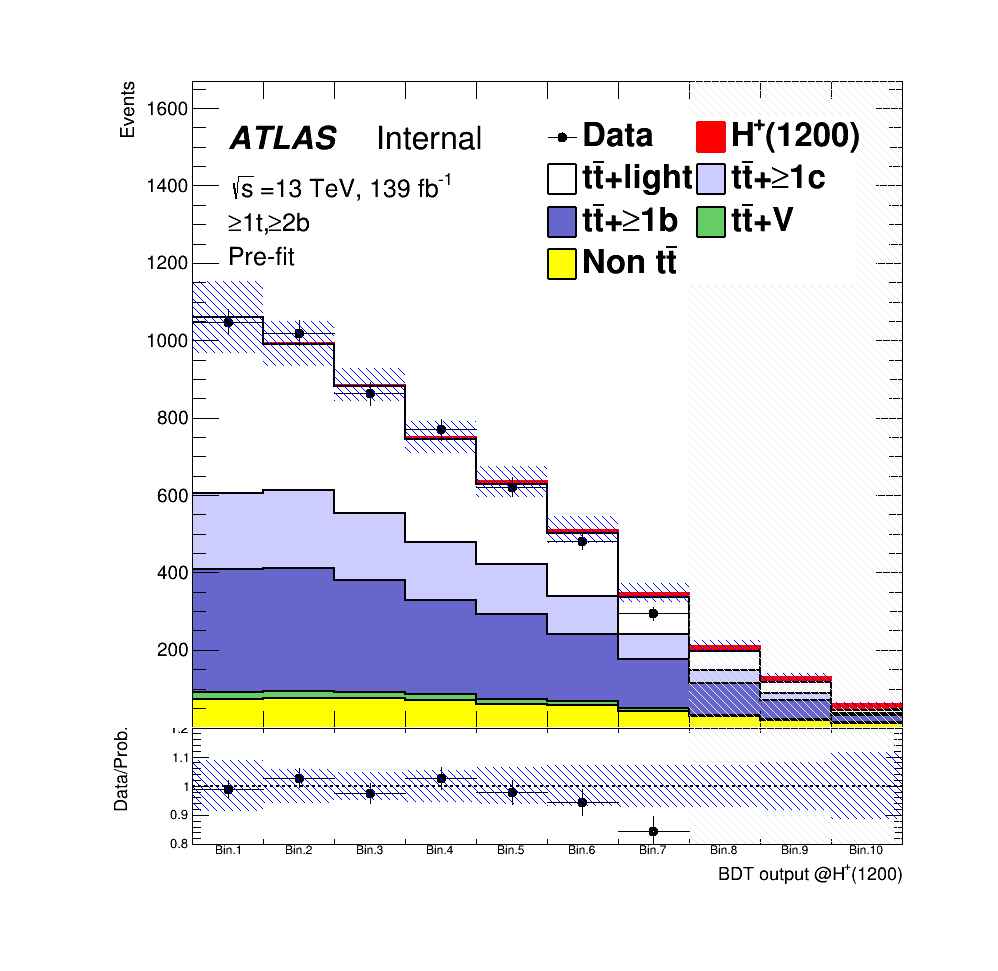
\includegraphics[width=0.50\textwidth]{images/BkgModeling/DATAOVERMC_Hp1200_Contained80_DL1r_70_bdt_Hp1200_geq1tgeq2b_prefit.png}
    \label{fig:Prefit_BDT_Hp1200}
  }
  \subfloat[] {
    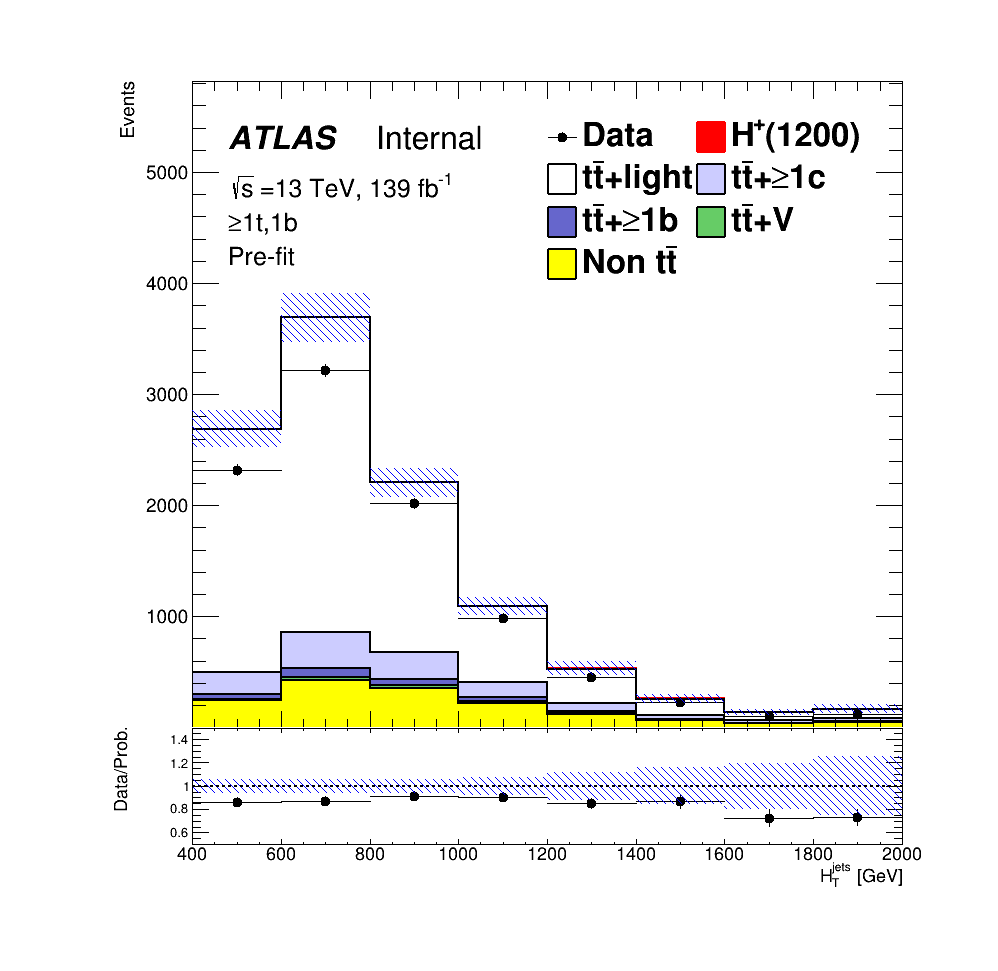
\includegraphics[width=0.50\textwidth]{images/BkgModeling/DATAOVERMC_Hp1200_Contained80_DL1r_70_HT_jets_geq1t1b_prefit.png}
    \label{fig:Prefit_HT_jets_Hp1200}
  }
  \caption{Pre-fit distribution of BDT output in the SR (a) and $H_{\text{T}}^{\text{jets}}$ in the CR for the 1200 GeV $H^{+}$ mass hypotheses.}
  \label{fig:Prefit_Hp1200}
\end{figure}

\begin{figure}[H]
  \subfloat[] {
    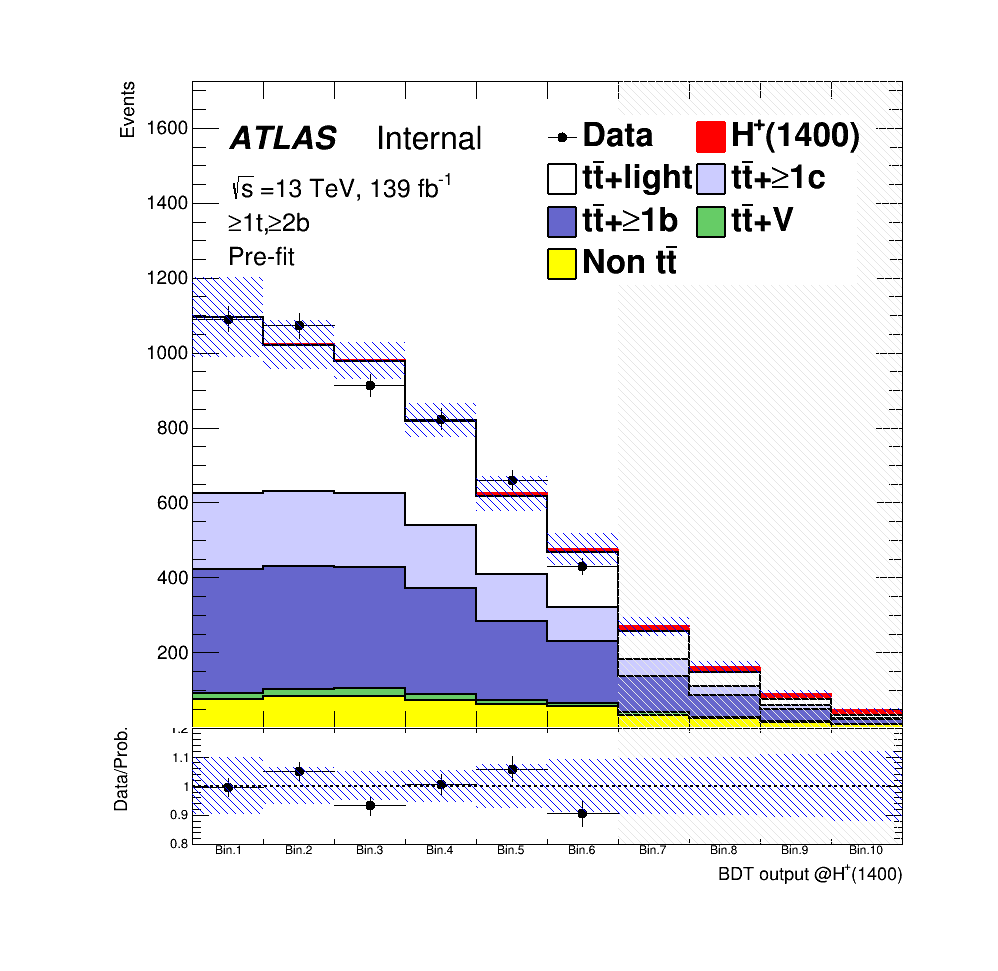
\includegraphics[width=0.50\textwidth]{images/BkgModeling/DATAOVERMC_Hp1400_Contained80_DL1r_70_bdt_Hp1400_geq1tgeq2b_prefit.png}
    \label{fig:Prefit_BDT_Hp1400}
  }
  \subfloat[] {
    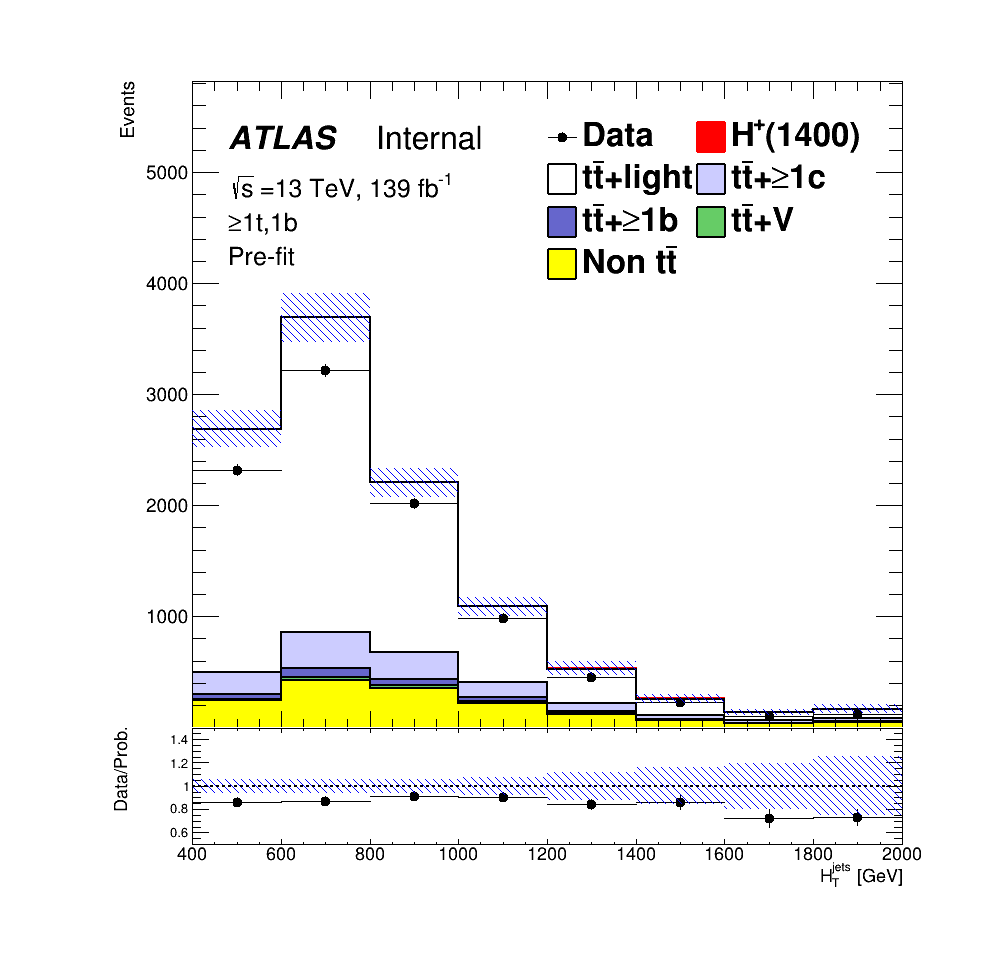
\includegraphics[width=0.50\textwidth]{images/BkgModeling/DATAOVERMC_Hp1400_Contained80_DL1r_70_HT_jets_geq1t1b_prefit.png}
    \label{fig:Prefit_HT_jets_Hp1400}
  }
  \caption{Pre-fit distribution of BDT output in the SR (a) and $H_{\text{T}}^{\text{jets}}$ in the CR for the 1400 GeV $H^{+}$ mass hypotheses.}
  \label{fig:Prefit_Hp1400}
\end{figure}

\begin{figure}[H]
  \subfloat[] {
    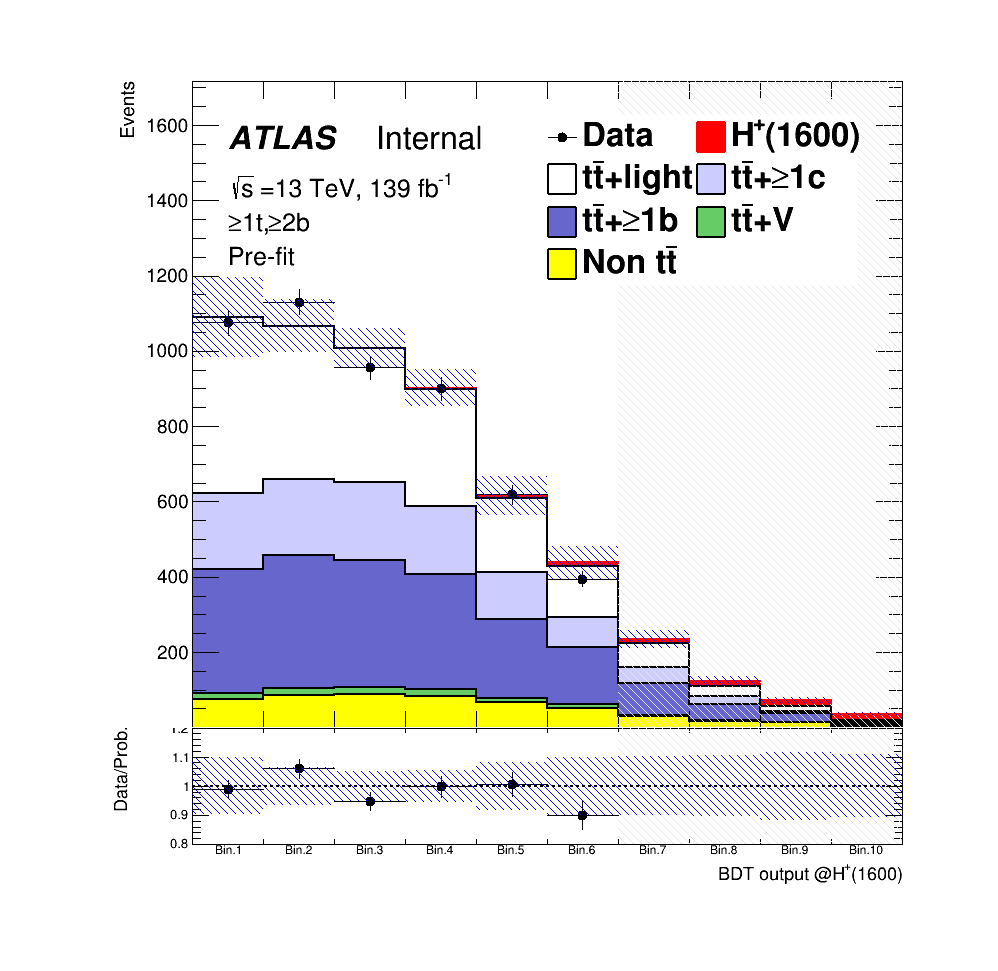
\includegraphics[width=0.50\textwidth]{images/BkgModeling/DATAOVERMC_Hp1600_Contained80_DL1r_70_bdt_Hp1600_geq1tgeq2b_prefit.png}
    \label{fig:Prefit_BDT_Hp1600}
  }
  \subfloat[] {
    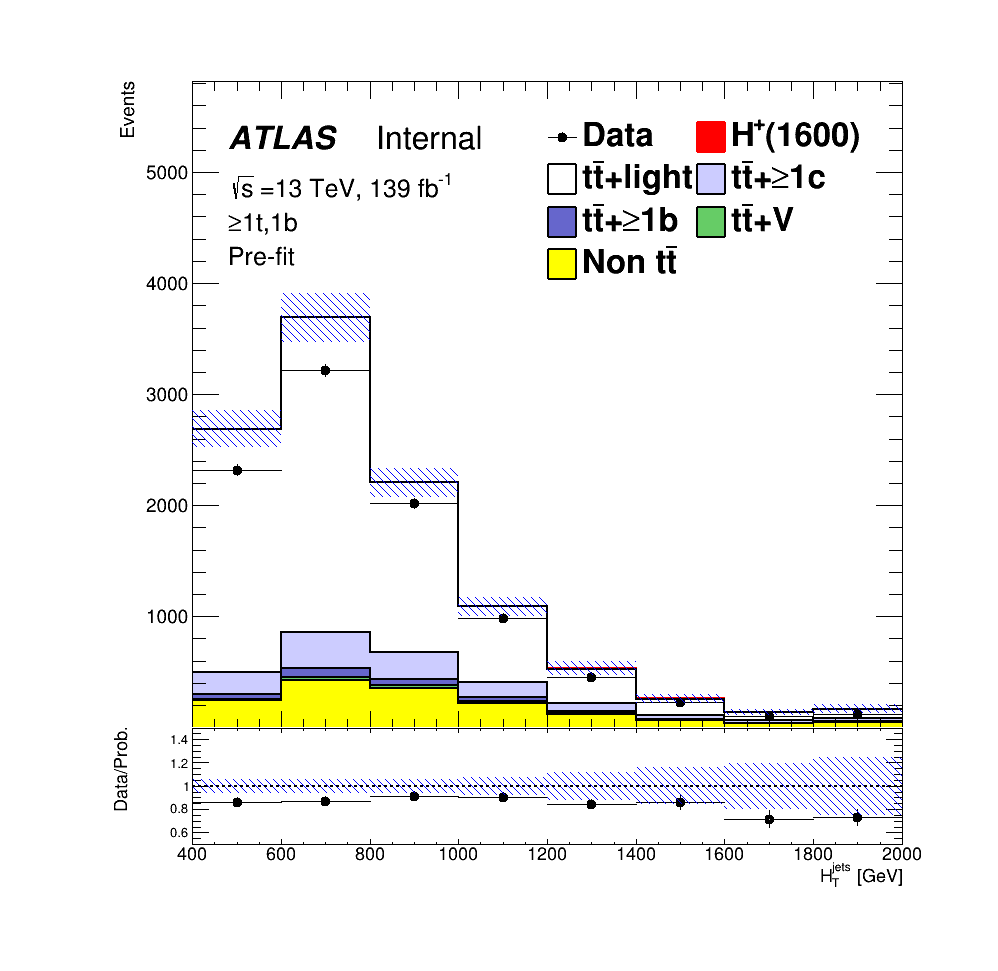
\includegraphics[width=0.50\textwidth]{images/BkgModeling/DATAOVERMC_Hp1600_Contained80_DL1r_70_HT_jets_geq1t1b_prefit.png}
    \label{fig:Prefit_HT_jets_Hp1600}
  }
  \caption{Pre-fit distribution of BDT output in the SR (a) and $H_{\text{T}}^{\text{jets}}$ in the CR for the 1600 GeV $H^{+}$ mass hypotheses.}
  \label{fig:Prefit_Hp1600}
\end{figure}

\begin{figure}[H]
  \subfloat[] {
    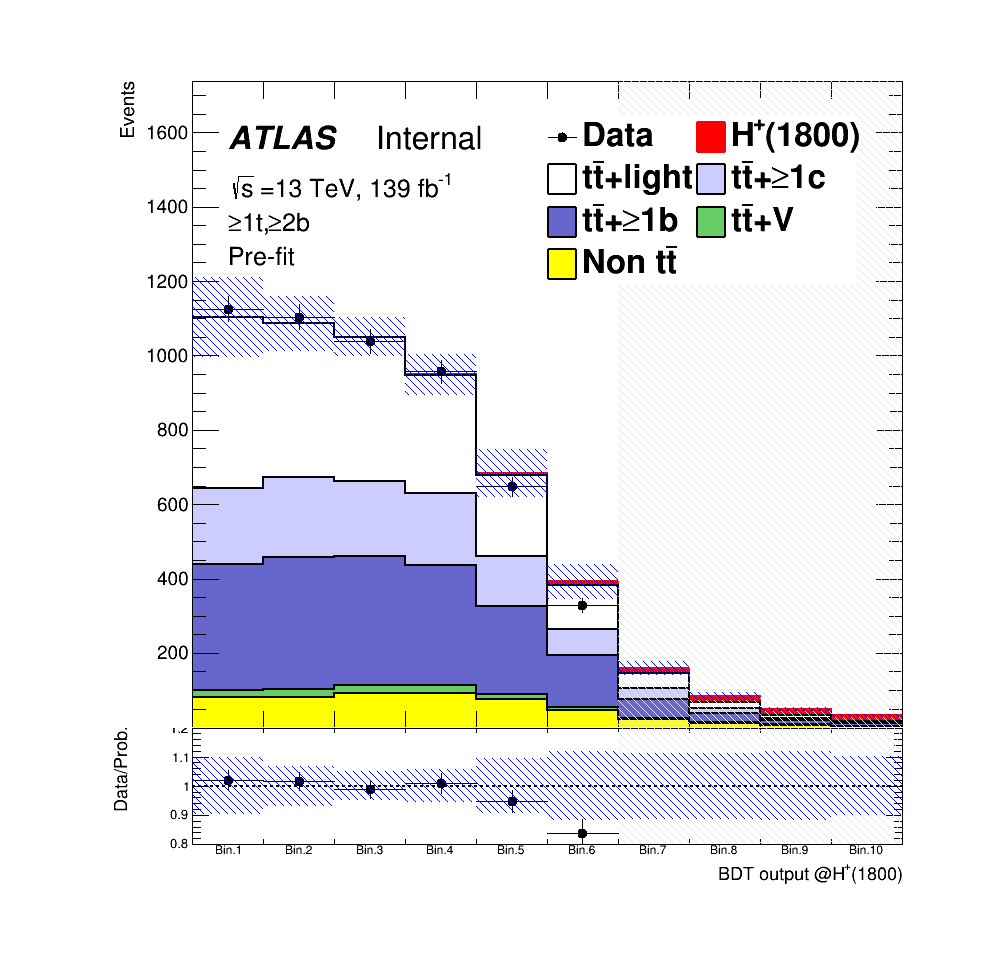
\includegraphics[width=0.50\textwidth]{images/BkgModeling/DATAOVERMC_Hp1800_Contained80_DL1r_70_bdt_Hp1800_geq1tgeq2b_prefit.png}
    \label{fig:Prefit_BDT_Hp1800}
  }
  \subfloat[] {
    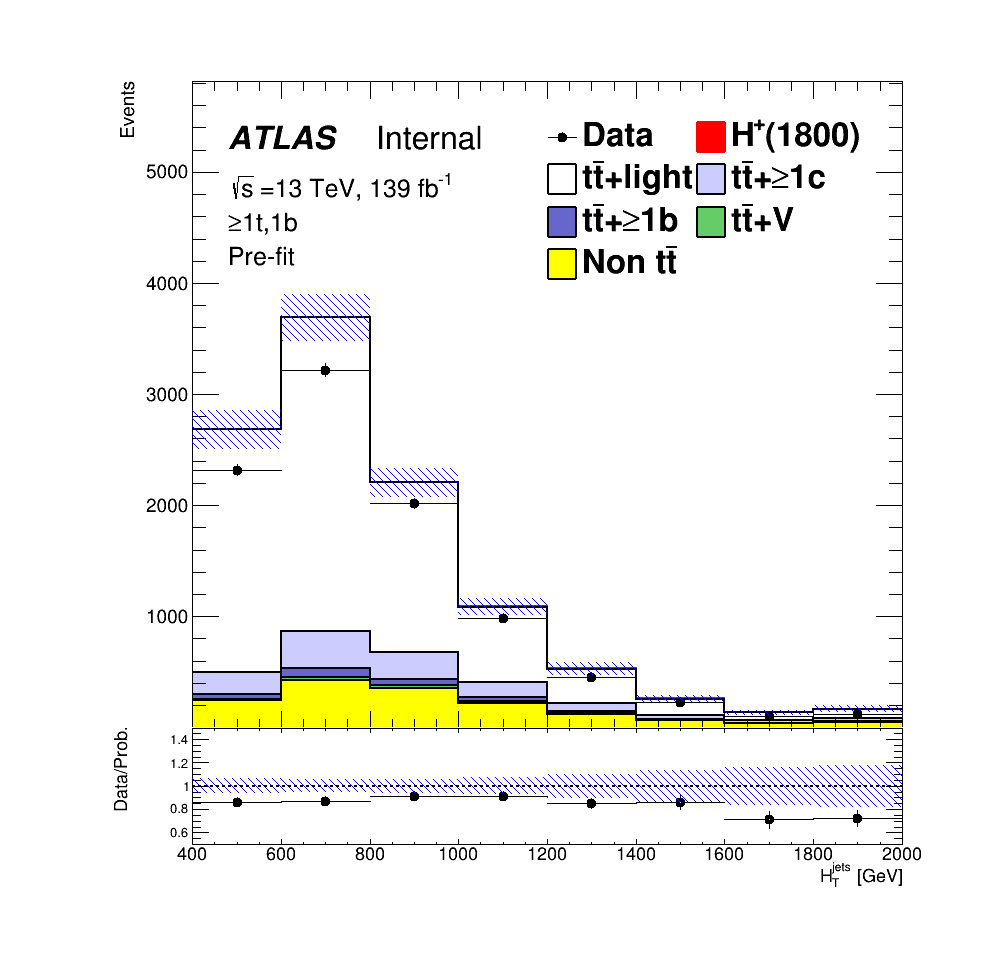
\includegraphics[width=0.50\textwidth]{images/BkgModeling/DATAOVERMC_Hp1800_Contained80_DL1r_70_HT_jets_geq1t1b_prefit.png}
    \label{fig:Prefit_HT_jets_Hp1800}
  }
  \caption{Pre-fit distribution of BDT output in the SR (a) and $H_{\text{T}}^{\text{jets}}$ in the CR for the 1800 GeV $H^{+}$ mass hypotheses.}
  \label{fig:Prefit_Hp1800}
\end{figure}

\begin{figure}[H]
  \subfloat[] {
    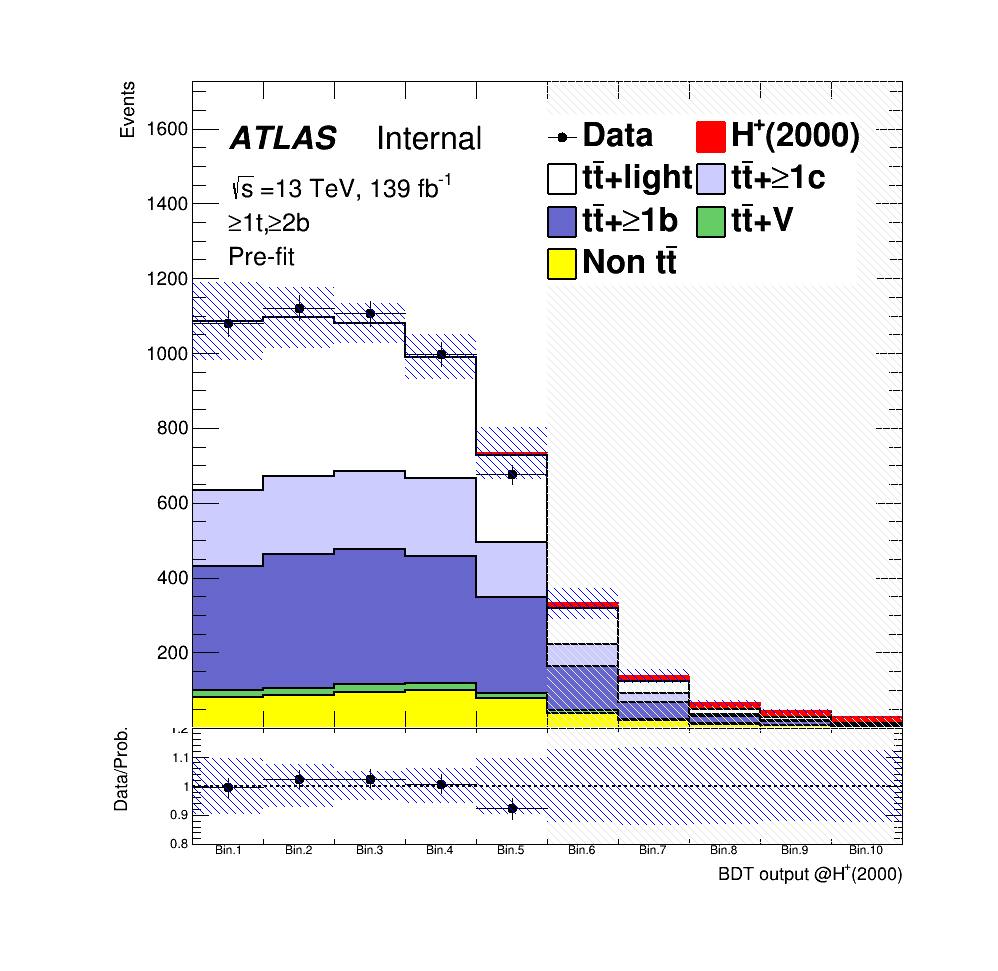
\includegraphics[width=0.50\textwidth]{images/BkgModeling/DATAOVERMC_Hp2000_Contained80_DL1r_70_bdt_Hp2000_geq1tgeq2b_prefit.png}
    \label{fig:Prefit_BDT_Hp2000}
  }
  \subfloat[] {
    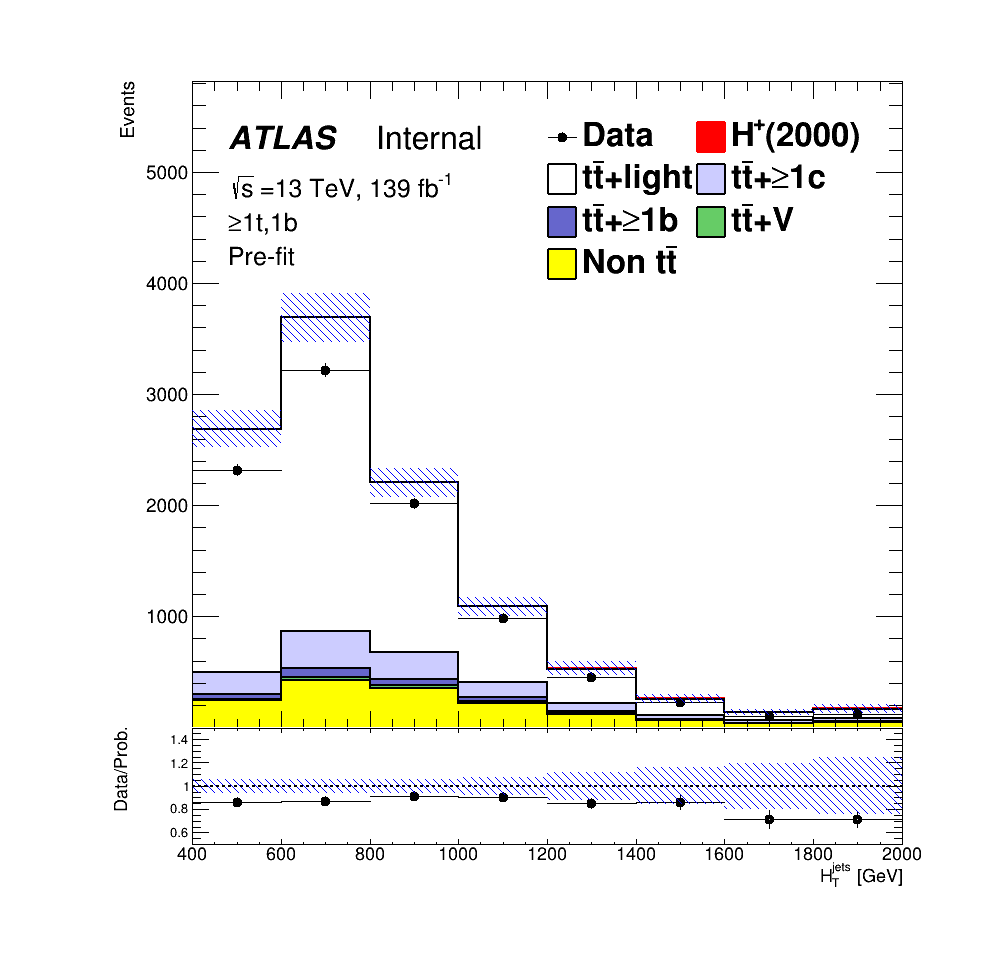
\includegraphics[width=0.50\textwidth]{images/BkgModeling/DATAOVERMC_Hp2000_Contained80_DL1r_70_HT_jets_geq1t1b_prefit.png}
    \label{fig:Prefit_HT_jets_Hp2000}
  }
  \caption{Pre-fit distribution of BDT output in the SR (a) and $H_{\text{T}}^{\text{jets}}$ in the CR for the 2000 GeV $H^{+}$ mass hypotheses.}
  \label{fig:Prefit_Hp2000}
\end{figure}

\begin{figure}[H]
  \subfloat[] {
    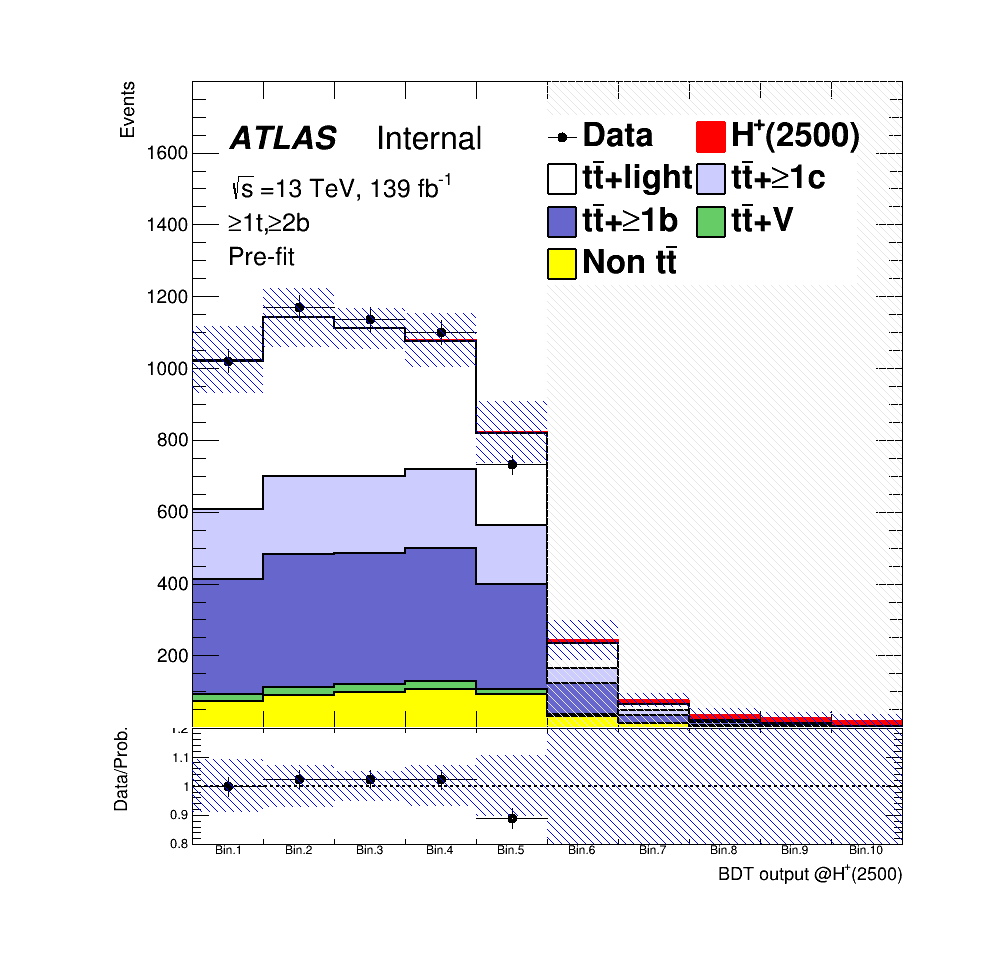
\includegraphics[width=0.50\textwidth]{images/BkgModeling/DATAOVERMC_Hp2500_Contained80_DL1r_70_bdt_Hp2500_geq1tgeq2b_prefit.png}
    \label{fig:Prefit_BDT_Hp2500}
  }
  \subfloat[] {
    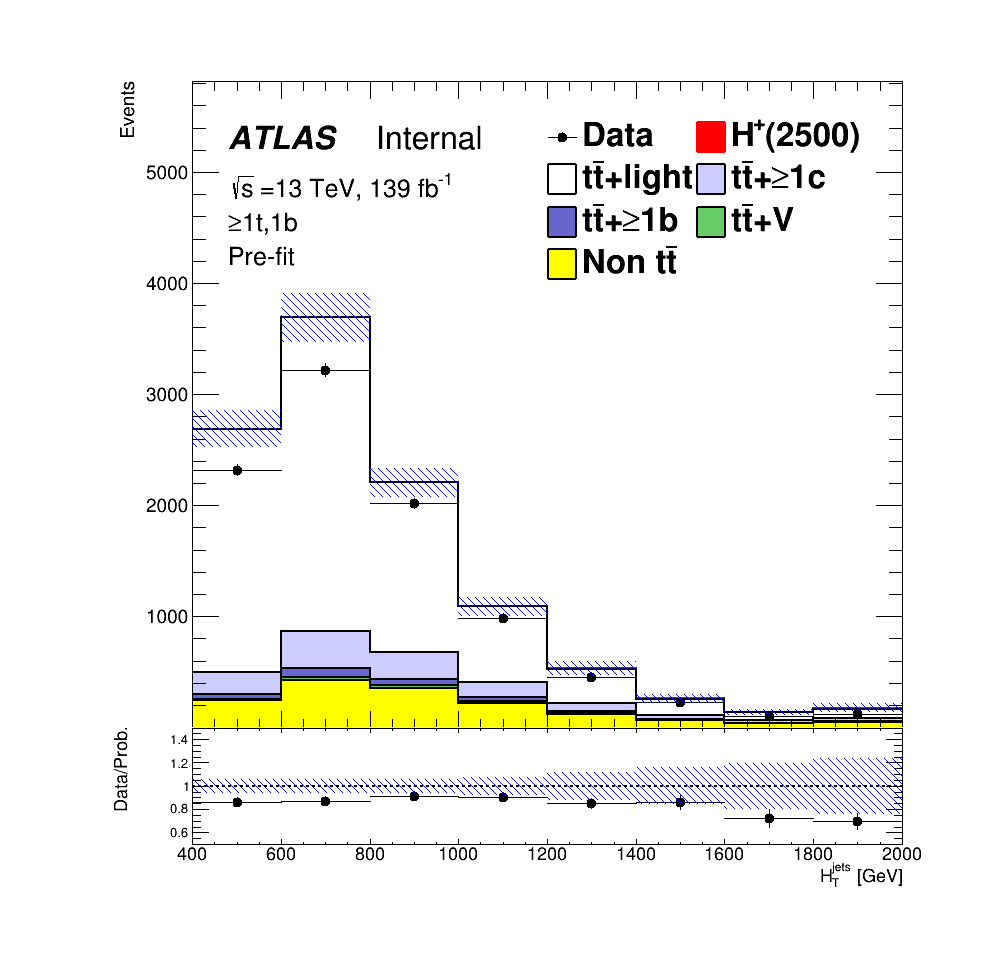
\includegraphics[width=0.50\textwidth]{images/BkgModeling/DATAOVERMC_Hp2500_Contained80_DL1r_70_HT_jets_geq1t1b_prefit.png}
    \label{fig:Prefit_HT_jets_Hp2500}
  }
  \caption{Pre-fit distribution of BDT output in the SR (a) and $H_{\text{T}}^{\text{jets}}$ in the CR for the 2500 GeV $H^{+}$ mass hypotheses.}
  \label{fig:Prefit_Hp2500}
\end{figure}

\begin{figure}[H]
  \subfloat[] {
    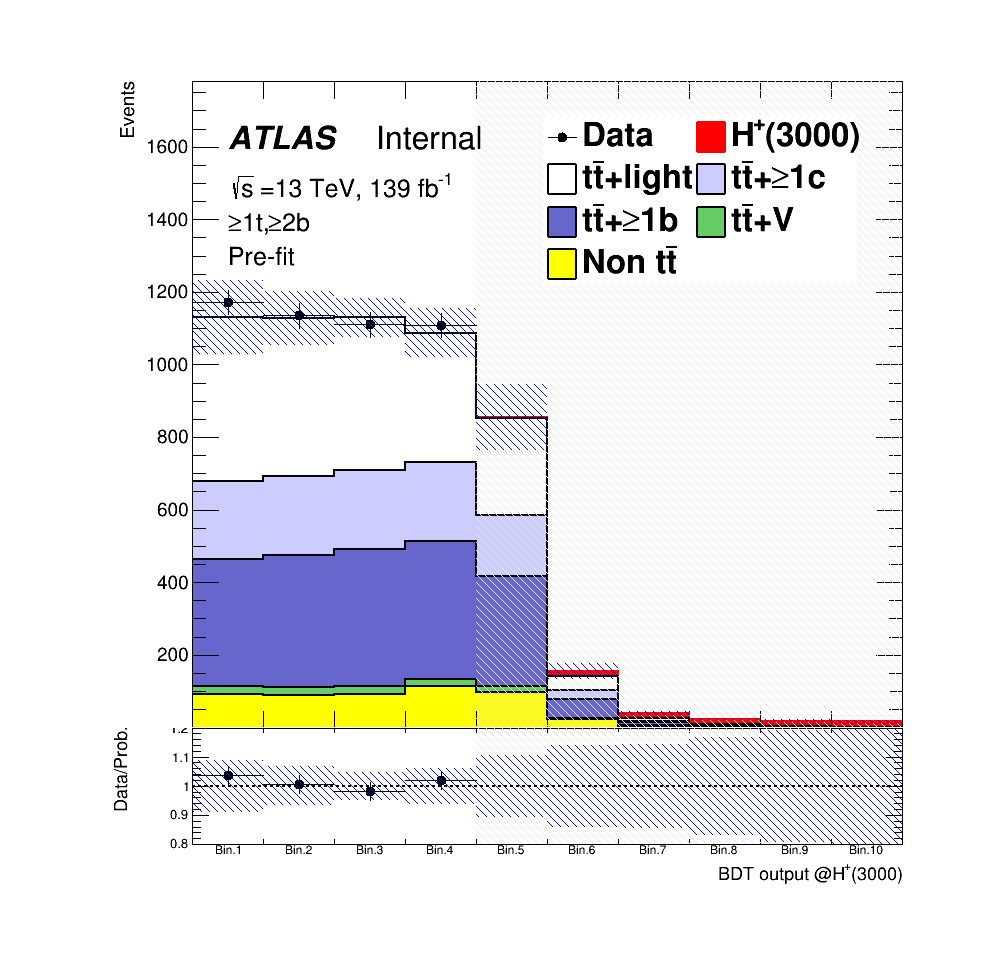
\includegraphics[width=0.50\textwidth]{images/BkgModeling/DATAOVERMC_Hp3000_Contained80_DL1r_70_bdt_Hp3000_geq1tgeq2b_prefit.png}
    \label{fig:Prefit_BDT_Hp3000}
  }
  \subfloat[] {
    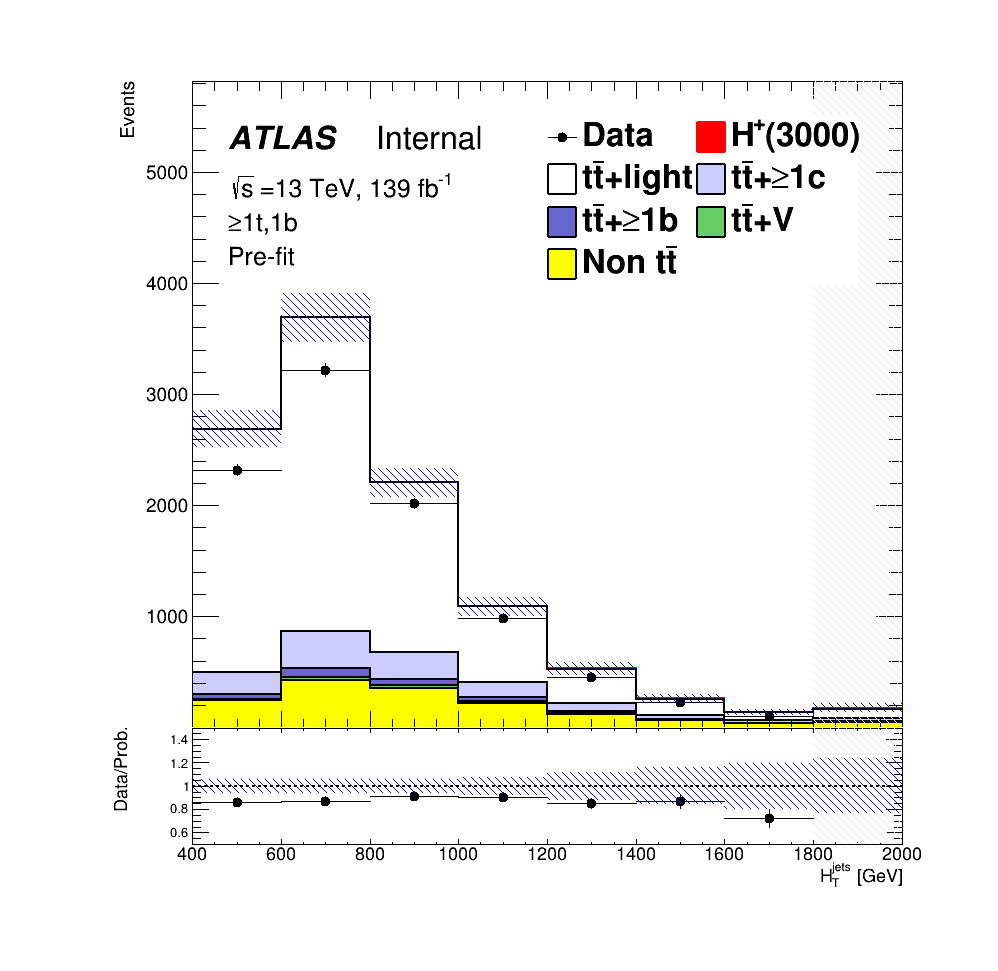
\includegraphics[width=0.50\textwidth]{images/BkgModeling/DATAOVERMC_Hp3000_Contained80_DL1r_70_HT_jets_geq1t1b_prefit.png}
    \label{fig:Prefit_HT_jets_Hp3000}
  }
  \caption{Pre-fit distribution of BDT output in the SR (a) and $H_{\text{T}}^{\text{jets}}$ in the CR for the 3000 GeV $H^{+}$ mass hypotheses.}
  \label{fig:Prefit_Hp3000}
\end{figure}

